\documentclass[../main.tex]{subfiles}
\begin{document}

% Kapitel Security Benchmarks?
%   \cite[S.36]{presContainerDockerSec}

% Kapitel Security Policies/Guidelines
%   \cite[S.37]{presContainerDockerSec}

% Aufbauen a la (Prozesse auflisten, un einzeln security features davon erklaeren):
%   1. ISO Download
%   2. Verify check sums
%   3. Install OS
%   4. Prepare OS for imaging
%   5. Create Docker image
%   6. Upload to internal registry server
%   7. Share with others

\chapter{Sicherheit im Docker-Ökosystem}
\label{secEcosystem}
  In diesem Kapitel werden einige Anwendungsaspekte von Docker unter einem Sicherheitskontext beleuchtet. Maßgeblich sollen weiterhin die drei definierten Sicherheitsziele zur Bewertung von Sicherheitseigenschaften dienen. Während Kapitel \ref{secLinux} native Sicherheitskomponenten von Docker und Linux untersucht hat, wird in den folgenden Abschnitten das Docker-Ökosystem in Betracht gezogen. Unter einem Ökosystem versteht sich hierbei die Gesamtheit aller Komponenten und Interaktionsmöglichkeiten, die im Zusammenhang mit Docker existieren. Der Fokus der Untersuchung liegt auf Anwendungsebene. Das bedeutet, dass hauptsächlich Methoden vorgestellt werden, die Docker Entwicklern und Administratoren zur Verfügung stellt, um die Arbeit mit den Docker-Komponenten aus Kapitel \ref{dockerIntro} sicher zu gestalten. Außerdem wird vorgestellt, wie sich die sicherheitsrelevanten Komponenten und Operationen in den letzten Monaten aus der Sicherheitsperspektive geändert haben.

  % TODO: Erwaehnen, das Fokus auf erst neulich hinzugefuegten, aktuell entwickelten und zukünftig geplanten Features liegt.

  Die Untersuchung sieht folgende Themen vor:

  \begin{itemize}
    \item Verbindung zwischen Docker-Client und Docker-Daemon
    \item Verwaltung von Images
    \item Betrieb von Containern
    \item Verwendung von Plugins
    \item Verwendung von 3rd-Party-Tools, wie z.B. Kubernetes
  \end{itemize}

  % Je nach Vorankommen, können hier ganze Sektions weggelassen werden imo.
  % Tendenziell mehr die Themen zuerst, die direkt mit Security zu tun haben.
  % Auch Fokus auf die neusten Entwicklungen (2015 und 2016) in Sachen Sicherheit und neue Docker-Features

  % High level goals of docker project to improve security
  % • Map root user of the container to non-root user of docker
  % • Make docker daemon run as a non root user
  % ^   \cite[S.3]{virtVSContainer}

  % Support for TUF Delegations: Docker now has support for read/write TUF delegations, and as soon as notary 0.2 comes out, you will be able to use delegations to provide signing capabilities to a team of developers with no shared keys.
  %   ^   \cite{https://news.ycombinator.com/item?id=11037543}

  \section{Private Registries}
    Docker bietet neben der Nutzung des öffentlichen Docker Hubs an, private Registries zu erstellen. Diese können dann, z.B. von einer Firewall gesichert oder von einem Load-Balancer unterstützt, in der firmeneignen Infrastruktur oder in Rechenzentren externer Public-Cloud-Anbieter betrieben werden. Für Cloud-Anbieter stellt Docker einige Speichertreiber zur Verfügung, z.B. für Amazons S3 \cite{dockerStorageDriverS3}, Microsofts Azure \cite{dockerStorageDriverAzure}, und OpenStacks Swift \cite{dockerStorageDriverSwift}. Bei Bedarf können eigene Speichertreiber mit der \emph{Storage-API} implementiert werden \cite{dockerStorageDriver}.
    % \cite[S.5]{dockerSecIntro}
    Neben der Vertraulichkeit von Images, bieten private Registries den Vorteil, dass sich die Speicherung und Verteilung von Images an den internen und häufig durch \emph{Continuous Integration} und \emph{Continuous Delivery} automatisierten Softwareentwicklungsprozess anpassen lassen. Registries selbst können als Container betrieben werden \cite{dockerRegistry}.
    % TODO: CI/CD im Glossar definieren

    Außerdem lässt sich das öffentliche Docker Hub in einer privaten Registry spiegeln. Bei dem Herunterladen von Images aus der öffentlichen Registry, kann somit auf eine externe Verbindung verzichtet werden, sofern die Spiegelung in Form einer privaten Registry im eigenen Netz existiert. Docker kann mit der Option \texttt{--registry-mirror=ADDRESS} angewiesen werden, anstelle des Docker Hubs eine Spiegelung zu verwenden \cite{dockerRegistryMirror}.

    Der Zugriff auf eine Registry kann z.B. über \acrshort{HTTPS} und der Verwendung von Zertifikaten abgesichert werden \cite{dockerRegistry} (vgl. Kapitel \ref{conClientServer}).

  \section{Verfikation und Verteilung von Images}
    Der Sicherheitsforscher Jonathan Rudenberg hat im Dezember 2014 drei Sicherheitsrisiken im Zusammenhang mit Dockers damaliger Verifikation und Verteilungs von Images aufgedeckt \cite{githubRegistryV1Issues}\cite{registryV1IssuesRudenberg}. U.a. ist es durch Verwendung des \texttt{docker pull}-Befehls möglich manipulierte Images zu beziehen, die bereits beim Entpacken auf dem lokalen System beliebige Dateien im Hostsystem überschreiben können \cite{registryV1IssuesRedHat}. Sowohl die Integrität von Daten als auch die Verfügbarkeit der Hosts sind durch eine solche Gefahr direkt gefährdet. Auch die Aktualität von Images, sowie die Authenzität von Personen und Organisationen, die Images veröffentlichen, kann darunter leiden, wie in Kapitel \ref{tuf} zu sehen ist.

    In Docker wurden seit Version 1.8 schrittweise Mechanismen implementiert, die die Verifikation einerseits und das Verteilungsmodell von Images verbessern sollen. Diese umgesetzten, teilweise sich überschneidenen Ansätze, sind im Folgenden in Aspekte der Verifikation und Aspekte der Verteilung aufgeteilt.

    \subsection{Verifikation von Images}
      Seit Februar 2016 mit der Veröffentlichung von Docker-Version 1.10 sind Images über deren Inhalt addressierbar. Auf Implementierungsebene bedeutet das, dass die Layer-IDs nicht wie zuvor zufällig generierte UUIDs repräsentieren, sondern als SHA256-Hashwerte, die über die Layerdaten gebildet werden, vorliegen \cite[S.16]{slideshareImageDistribution}. Der SHA256-Hashalgorithmus wird derzeit als kryptographisch sicher gesehen, was zur Folge hat, dass die generierten Layer-IDs kollisionssicher sind und damit als einmalig gelten. Durch die deterministische Natur von Hashfunktionen wird gleichzeitig eine Methode implementiert, die die Integrität von Layern sicherstellt. In der Praxis kann die Korrektheit von Layerdaten validiert werden, indem ein frisch berechneter Hash eines Layers mit dem referenzierten Hasheintrag in den Image-Metadaten, dem Manifest, verglichen wird. Die referenzierten Hashwerte der Layer sind im Manifest in Form eines Hashbaums strukturiert. Seit der Version 2 des Manifests, kann die Manifestdatei signiert werden, um auch die Integrität der Metadaten zu gewährleisten \cite{githubImageManifest21}.

      Die zuvor verwendeten UUIDs erfüllen die deterministische Eigenschaft nicht, da sie unabhängig von den Daten bei jeder Generierung zufällig auf Basis der PRNG-Implementierung in \emph{Golang} entstehen \cite{githubImageUUID}.

      % Exkurs, das UUID nicht sicher sind aber SHA256 schon .... UUID sind eigtl auch sicher, nur eben immer nicht-deterministisch...

      % Content Addressed Images: The new manifest format in Docker 1.10 is a full Merkle DAG, and all the downloaded content is finally content addressable.
      % Seit Version 1.10
      %   ^   \cite{https://news.ycombinator.com/item?id=11037543}

      % registry v2: content based layer IDs und signed image manifests
      % davor registry v1: abgesehen von https (nur kommunikation), kein integritaetscheck des inhalts von images. Ausserdem willkuerliche Image IDs
      %   ^   \cite[S.27]{presContainerDockerSec}

    \subsection{Integration von \emph{The Update Framework}}
    \label{tuf}
      Die Integrität von Images spielt auch bei der Verteilung von Images über Docker-Registries eine große Rolle.
      % Die Verifikation von Daten hat zum Ziel die Integrität dieser zu bestätigen. Die Integrität von Images spielt beim Herunterladen von Images von entfernten Registries eine wichtige Rolle.

      Im August 2015 wurde mit der Docker-Version 1.8 ein Paket- und Verteilungsmodell umgesetzt, das die von Rudenberg entdeckten Schwächen in der Bereitstellung von Images beheben soll \cite{dockerContentTrust}. Unter dem Featurenamen \emph{Docker Content Trust} integriert Docker das Model \emph{The Update Framework} (TUF) \cite{tufFramework}, welches Gefahrenquellen wie manipulierte Images, Replay- und MITM-Angriffe ausschließt. Die Sicherheit von TUF basiert auf der Signierung von Images, mit der anhand mehrerer kryptographischer Schlüssel die Integrität, Authenzität sowie Aktualität von Images sichergestellt wird. Die Verwendung dieses Features ist optional und kann mit der Umgebungsvariable \texttt{DOCKER\_CONTENT\_TRUST} gesteuert werden.

      \emph{Docker Content Trust} wird in Docker als Notary integriert. Der Notary implementiert das TUF in \emph{Golang} und bietet Erstellern von Inhalten die Möglichkeit ihre Daten zu signieren. Die signierten Daten können dann über einen Notary-Server zum Download angeboten werden \cite{githubNotary}\cite{dockerContentTrust}.

      % https://lwn.net/Articles/628343/
      % https://github.com/docker/docker/issues/9719
      % https://securityblog.redhat.com/2014/12/18/before-you-initiate-a-docker-pull/
      % https://titanous.com/posts/docker-insecurity

      % https://github.com/docker/notary
      % https://blog.docker.com/2015/08/content-trust-docker-1-8/
      % https://blog.docker.com/2015/08/docker-1-8-content-trust-toolbox-registry-orchestration/

  \section{Verbindung zwischen Daemon und Client}
  \label{conClientServer}
    Wie in Kapitel \ref{dockerArchitecture} dargestellt, werden Anweisungen von Docker-Clients an einen Docker-Daemon übertragen, der diese über eine REST-API empfängt. Standardmäßig findet diese Kommunikation seit Version 0.5.2 über einen nicht netzwerkfähigen UNIX-Socket statt \cite{dockerSecurity}.

    Eine Umgebung, die vorsieht Client und Daemon voneinander getrennt über ein Netzwerk zu betreiben, benötigt jedoch einen HTTP-Socket, um die Konnektivität der beiden Komponenten über das Netzwerk zu gewährleisten.

    Obwohl die Netzwerksicherheit nicht Bestandteil dieser Arbeit ist, werden die Mechanismen, die Docker zur Absicherung der Kommunikation zwischen Client und Daemon unterstützt, kurz vorgestellt.

    Mittels eigener Zertifikate können sich Daemon und Clients gegenseitig sicher über HTTPS authentifizieren. Unbefugte, fremde Daemons oder Clients können dadurch nicht mit einem vertrauenswürdigen Komplementär interagieren. Die Authentifizierung kann demnach uni- oder bidirektional erfolgen. Durch die sichere Kommunikation mittels HTTPS, das auf dem Protokoll TLS basiert, erfüllen die zu übermittelnden Daten die Sicherheitsziele Vertraulichkeit und Integrität.

    Die entsprechende Konfiguration eines Daemons kann z.B. mit dem Befehl \texttt{docker daemon --tlsverify --tlscacert=CA.pem --tlscert=SERVER-CERT.pem --tlskey=SERVER-KEY.pem} vorgenommen werden. Analog dazu erfolgt die clientseitige Einstellung über \texttt{docker --tlsverify --tlscacert=CA.pem --tlscert=CERT.pem --tlskey=KEY.pem COMMAND}. Der Parameter \texttt{--tlsverify} gibt jeweils an, dass der Kommunikationspartner authentifiziert werden muss. Die Authenfikation geschieht über die Parameterwerte \texttt{--tlscert} und \texttt{--tlskey} des Kommunikationspartners, die zusammen die Identität dessen bekannt geben. Unter Angabe eines CA-Zertifikats mit Parameter \texttt{--tlscacert} hat die Authentifizierung nur dann Erfolg, wenn das Zertifikat des Kommunikationspartners von dieser CA ausgestellt wurde \cite{dockerSecurityHTTPS}. In einer Unternehmensinfrastruktur kann so die Kommunikation durch eine unternehmenseigene CA weiter restriktiviert werden. Eine detailreichere Beschreibung der verschiedenen Betriebsmodi ist unter \cite{dockerSecurityHTTPS} gegeben.

    Über die Umgebungsvariable \texttt{DOCKER\_TLS\_VERIFY} sowie der Speicherung der notwendigen Zertifikate und Schlüssel unter \texttt{.docker/} im Homeverzeichnis, kann die Konfiguration der Authentifizierung einmalig für die zukünftige Kommunikation vorgenommen werden \cite{dockerSecurityHTTPS}.

    % https://docs.docker.com/engine/security/security/
    % https://docs.docker.com/engine/security/https/

    % Secure communications is also vital to building and shipping applications, as container images are in constant change and need to be pushed and pulled through your infrastructure. All communications with the registries use TLS, to ensure both confidentiality and content integrity. By default, the use of certificates trusted by the public PKI infrastructure is mandatory, but Docker allows the addition of a company internal CA root certificate to the truststore.
    %   ^   \cite[S.5]{dockerSecIntro}

    % TODO: An anderer Stelle im Überblick erwähnen, dass in diesem speziellen Unterkapitel kurz auf Netzwerksicherheit eingegangen wird. Halt nur docker-spezifische Netzwerksicherheit.

  \section{Docker Plugins}
  \label{plugins}
    Seit Juni 2015 unternahmen die Entwickler von Docker Anstrengungen, um optionale Komponenten von Docker in eine eigene Plugin-Infrastruktur zu integrieren, in der Plugins modular aktiviert und deaktiviert werden können \cite{githubDockerChangelog}\cite{dockerPlugins}. Plugins werden von einem Docker-Daemon genutzt und erweitern dessen Fähigkeiten. Neben den ersten Plugins für diverse Netzwerkfunktionen, z.B. \emph{Weave}, und der Einbindung von Datenträgern, z.B. \emph{Flocker}, fand im Frühjahr 2016 mit Docker-Version 1.10 auch ein ursprünglich von \emph{Twistlock}\cite{twistlock} entwickeltes Authorisierungs-Plugin Einzug in Docker, das in diesem Kapitel zur Vereinfachung auch als \emph{AuthZ} bezeichnet wird \cite{githubPluginList}\cite{dockerPlugins}\cite{authzTwistlock}.

    Ergänzend dazu war auch ein Authentifizierungs-Plugin \emph{AuthN} geplant, das Nutzer vor deren Authorisierung durch \emph{AuthZ}, authentifiziert \cite{githubAuthZDockerAccessControl}. Am 23. Februar 2016 hat jedoch ein Docker-Mitarbeiter bekannt gegeben, dass die Integration von \emph{AuthN} eingestellt wird. Grund hierfür ist, dass die Authentifizierung - nach der Meinung einiger Docker-Entwickler - leicht außerhalb des Daemons stattfinden kann, z.B. mit dem Authentifizierungsdienst Kerberos\cite{kerberos} \cite{githubAuthZKerberosSupport}\cite{githubAuthNLaydown}.

    Das Sicherheitsplugin \emph{AuthZ} hat zum Ziel ein Framework bereitzustellen, über das es Administratoren möglich ist, eine nutzer- und rollenbasierte Sicherheitspolitik umzusetzen. Diese umfasst Regeln, die die Benutzung des Docker-Daemons betreffen. Nach der ursprünglichen Implementierung von \emph{Twistlock} sind die Regeln in eine JSON-Struktur gefasst \cite{githubAuthZJSON}. Ohne ein solches Plugin ist jedem Nutzer, der den Docker-Daemon ausführen kann, die komplette Kontrolle über das Docker-System gegeben. V.a. in Unternehmen macht es aber Sinn, verschiedenen Nutzer im Rahmen eines RBAC-Sicherheitsmodells eine bestimmte Rolle zuzuweisen, die deren Rechte definiert. Ein einfacher Anwendungsfall könnte folgende Regeln beinhalten \cite{authzTwistlock}:
    % TODO: Einarbeiten: Abbildung administrativer Sicherheitsmodelle (durch technische Mechanismen?)

    \begin{itemize}
        \item User in der Gruppe \emph{Operations} dürfen nur Container starten und stoppen. Sie sollen nur \texttt{docker run CONTAINER} und \texttt{docker rm CONTAINER} ausführen können.
        \item User in der Gruppe \emph{Audit} dürfen nur Informationen von Images und Containern abfragen. Sie sollen nur \texttt{docker inspect IMAGE|CONTAINER} ausführen können.
        \item User \emph{Admin} darf jede Operation \texttt{docker ...} über den Daemon ausführen.
    \end{itemize}

    Aus Sicht der Architektur funktioniert die Authorisierung, wie sie in \fig \ref{fig:sec_authz} illustriert ist. Die Anfragen von lokalen oder entfernten Clients werden, wie in Kapitel \ref{dockerArchitecture} beschrieben, an einen Daemon geschickt. Dieser führt nun nicht die Befehle der Clients umgehend aus, sondern leitet die Anfrage an das \emph{AuthZ}-Framework weiter. Genauer erhält \emph{AuthZ} einen Nutzerkontext und einen Befehlskontext, die, z.B. anhand der zuvor definierten Regeln, ausgewertet werden. Anhand der dem Plugin vorliegenden Parameter entscheidet es, ob der Nutzer berechtigt ist, den angefragten Befehl auszuführen. Falls das nicht der Fall ist, wird eine Fehlernachricht über den Daemon an den Client gesendet (vgl. \fig \ref{fig:sec_authzDeny}). Falls die Anfrage genehmigt wurde, führt der Daemon den darin enthaltenen Befehl aus, und kontaktiert das Plugin ein zweites Mal mit dem Ergebnis des ausgeführten Befehls (vgl. \fig \ref{fig:sec_authzAllow}). \emph{AuthZ} hat hierbei die Gelegenheit, die Antwort, bevor sie zum Client gesendet wird, zu modifizieren \cite{githubAuthZDraft}\cite{authzTwistlock}.

    %\begin{figure}[h]
        %\centering
        %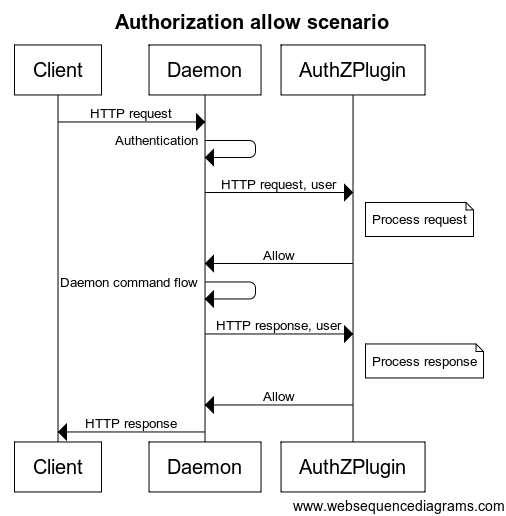
\includegraphics[width=0.9\textwidth]{./images/sec_authzAllow.png}
        %\caption{Ablaufdiagramm einer Befehlsausführung mit \emph{AuthZ} im Fall einer erfolgreichen Authorisierung \cite{githubAuthZExtended}.}
        %\label{fig:sec_authzAllow}
    %\end{figure}

    %\begin{figure}[h]
        %\centering
        %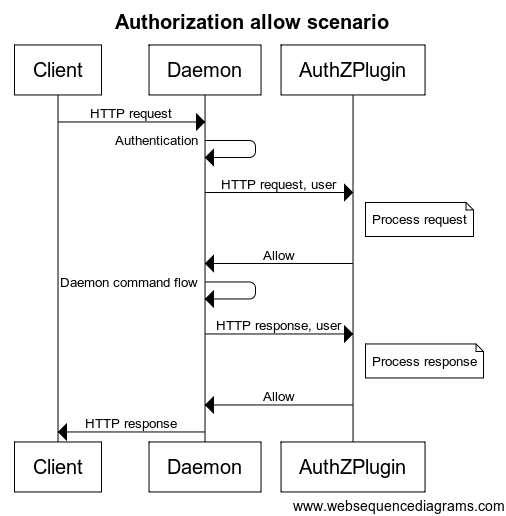
\includegraphics[width=0.9\textwidth]{./images/sec_authzAllow.png}
        %\caption{Ablaufdiagramm einer Befehlsausführung mit \emph{AuthZ} im Fall einer fehlgeschlagenen Authorisierung \cite{githubAuthZExtended}.}
        %\label{fig:sec_authzDeny}
    %\end{figure}

    \begin{figure}
      \centering
      \begin{subfigure}{.5\textwidth}
        \centering
        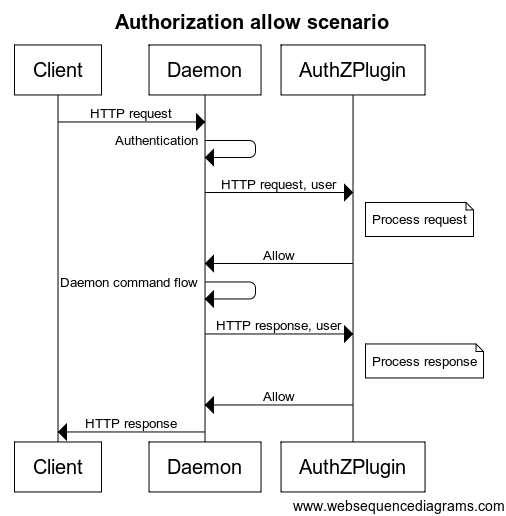
\includegraphics[width=1.0\linewidth]{./images/sec_authzAllow.png}
        \caption{Erfolgreiche Authorisierung}
        \label{fig:sec_authzAllow}
      \end{subfigure}%
      \begin{subfigure}{.5\textwidth}
        \centering
        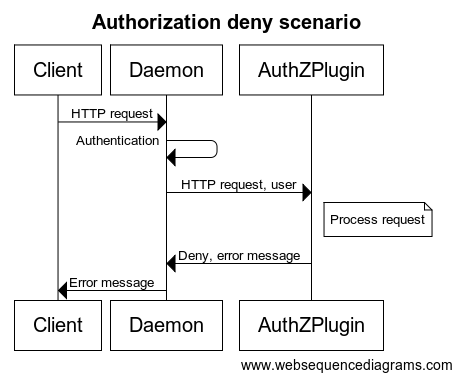
\includegraphics[width=1.0\linewidth]{./images/sec_authzDeny.png}
        \caption{Fehlgeschlagene Authorisierung}
        \label{fig:sec_authzDeny}
      \end{subfigure}
      \caption{Ablaufdiagramm einer Befehlsausführung mit dem Authorisierungs-Plugins \emph{AuthZ} von Docker \cite{githubAuthZExtended}.}
      \label{fig:sec_authz}
    \end{figure}
    % TODO: Evtl. untereinander machen da zu wenig Platz. Oder Grafik neu machen mit weniger/groesserem Text

    Die Formate von Anfragen und Antworten, die über das HTTP-Protokoll ausgetauscht werden, sind in \cite{githubAuthZExtended} spezifiziert.

    Mehrere Sicherheitsmodule können konsekutiv ausgeführt werden, sodass jede clientseitige Interaktion mit dem Daemon, die Ausführung mehrerer \emph{AuthZ}-Implementierungen zur Folge hat.

    Mit folgender Syntax können Authorisierungs-Plugins für den Daemon aktiviert werden \cite{githubAuthZExtended}:

    \begin{lstlisting}
      docker daemon --authorization-plugin=PLUGIN1 \
                   [--authorization-plugin=PLUGIN2] [...]
    \end{lstlisting}

    Da es sich bei diesen sicherheitsrelevanten Plugins um ein sehr neues Feature von Docker handelt, war die offizielle Dokumentation zum Zeitpunkt der Erstellung dieser Arbeit nicht vollständig. V.a. die fehlende Spezifikation des Formats eines \emph{AuthZ}-Regelwerks im Docker-Repository lässt vermuten, dass eine vollständige Einführung von \emph{AuthZ} erst im Rahmen zukünftiger Docker-Releases stattfindet.

  \section{Open-Source-Charakter und Sicherheitspolitik von Docker}
  \label{opensource}
    Docker ist wie Linux ein Open-Source-Projekt, das nicht nur von Docker-Mitarbeitern entwickelt wird, sondern die Unterstützung vieler freiwilliger Entwickler und Sicherheitsexperten findet. Der Open-Source-Charakter von Docker und Software allgemein kann jedoch aus Sicherheitssicht kontrovers diskutiert werden:

    \paragraph{Vorteile:}
    \begin{itemize}
      \item Durch die Vielzahl an Involvierten können Sicherheitslücken schneller entdeckt und behoben werden. Über 1300 Individuen haben sich bislang für die Weiterentwicklung der Codebasis und der Aufdeckung von Fehlern und Sicherheitsrisiken an Docker beteiligt.
      %Die Codequalität profitiert auch von Experten anderer Unternehmen und Organisationen, im Docker-Projekt z.B. von \emph{RedHat}-Mitarbeitern.
      \item Eigene Sicherheitspraktiken können von Anwendern durch die Kenntnis über den Quellcode hinzugefügt werden.
      \item Nach dem Kerkhoffs'schen Prinzip ist einer Anwendung von \emph{Security Through Obscurity} generell abzuraten \cite[S.15]{nist}.
    \end{itemize}

    \paragraph{Nachteile:}
    \begin{itemize}
      \item Sicherheitslücken sind von Angreifern prinzipiell schneller zu finden, wenn diese im Besitz des Quellcodes sind.
      \item Außerdem ist durch die lose Zusammenarbeit vieler Experten nicht gewährleistet, dass bestimmte Implementierungen nach dem Mehraugenprinzip kontrolliert werden. Die böswillige Absicht nur eines Entwicklers kann in einer Open-Source-Kultur weiterhin fatale Be\-ein\-träch\-ti\-gung\-en der Sicherheit mit sich ziehen.
    \end{itemize}

    Die Vor- und Nachteile zeigen auf, dass es keinen Gewinner nach Maßstäben der Sicherheit gibt. Sowohl Open-Source- als auch proprietäre Softwarelösungen können erfolgreich sein, wie die Vergangenheit bekannter Betriebssysteme und Anwendungen zeigt. Für \emph{Docker} hat sich der Open-Source-Ansatz bislang bewährt.

    Um die Zusammenarbeit im Docker-Projekt zu organisieren, wurden Regeln und Konventionen formuliert, die auch die Sicherheit betreffen \cite{githubDockerContribution}. Zusammen mit den Sicherheitsrichtlinien aus der offiziellen Docker-Homepage, ergeben sich folgende weitere, sicherheitsrelevante Eigenschaften von Docker.

    \begin{itemize}
      \item Prinzip von \emph{Responsible Disclosure} wird, als Hauptbestandteil der Sicherheitspolitik von Docker, umgesetzt. Konform dazu, können entdeckte Schwachstellen jederzeit an security@docker.com kommuniziert werden \cite{dockerSecurityPortal}.
      \item Wartung einer zentralen \acrshort{CVE}-Datenbank, die bekannte Sicherheitsrisiken von Docker enthält. Die darin veröffentlichten Informationen erfüllen das Prinzip \emph{Responsible Disclosure} \cite{dockerCVEList}.
      \item Externe Sicherheitsfirmen werden vierteljährlich beauftragt, Sicherheitsaudits und Penetrationstests zur Kontrolle der Codebasis und Infrastruktur durchzuführen \cite[S.5]{dockerSecIntro}.
    \end{itemize}

  \section{Security Best-Practises}
    Es existieren Skripte, die die Docker-Umgebung nach eingehaltenen und nicht erfüllten Best-Practices für die Sicherheit überprüfen.

    Der bekannteste Vertreter ist \emph{Docker Bench} \cite{githubDockerBench}, welcher in das Docker-Projekt integriert ist und nach Aussagen der Entwickler auf Befunden des Sicherheitsberichts des unabhängigen \emph{Center for Internet Security} \cite{dockerBenchmarkCIS} beruht. Dieser Bericht ist im Mai 2015 entstanden und enthält sicherheitsrelevante Befunde zu Docker in der Version 1.6. Aktuellere Berichte zu moderneren Docker-Versionen existieren nicht.

    Die darin enthaltenen Kontrollen sind in einem eigenen Image als Shellskripte definiert. Zur Ausführung der Tests muss dieses Image als Container gestartet werden. Im Rahmen dieser Tests werden direkt über Shellbefehle abrufbare Parameter untersucht. Darunter sind z.B.:

    \begin{itemize}
      \item Rechte, Besitzer- und Gruppenzugehörigkeiten von Dateien und Verzeichnissen
      \item Docker- und Kernelversion
      \item Log- und Netzwerkeinstellungen
      \item TLS-Unterstützung
      \item \texttt{--priviledged}-Status von Containern
      \item Verwendung von Capabilities, \emph{AppArmor}- und \emph{SELinux}-Profilen
    \end{itemize}

    Die Tests sind unter \cite{githubDockerBenchTests} in ihrer aktuellsten Version im Detail veröffentlicht.

    \subsection{Datencontainer}
      Die von Werkzeugen wie \emph{Docker Bench} ausführbare Tests beschränken sich auf explizit abrufbare Parameter des Hosts und von Docker. In Server-Infrastrukturen existieren jedoch auch Sicherheitskriterien, deren Kontrolle nicht über Abfragen von Host- oder Docker-Einstellungen abzudecken ist. Insbesondere wirken sich Merkmale der Infrastuktur auf die Verfügbarkeit von Services sowie Wartbarkeit der Infrastruktur aus.

      Z.B. wird von \emph{Docker} empfohlen, eigene Datencontainer zu betreiben, über die Anwendungen ihren Zustand auf Datenebene persistieren können. Anwendungen können in diesem Szenario über mehrere Container hinweg auf den Datencontainer zugreifen, sofern letzterer Methoden implementiert, um Race-Conditions zu verarbeiten. Standardmäßig gehen Änderungen, die während dem Betrieb von Containern auftreten, verloren sobald der Container gestoppt wird. Diese Eigenschaft beruht auf der obersten Schicht eines Containers, dem RW-Layer, der bei Containerstart einem Image hinzugefügt wird. Dieser Layer ist unabhängig von dem zugrundeliegendem Image und existiert nur temporär zur der Laufzeit des Containers. Dieser Eigenschaft unterliegt auch der Datencontainer. Aus diesem Grund empfiehlt es sich, die Verzeichnisse von Datencontainern aus dem Hostsystem über Mountpoints einzubinden. Welche Verzeichnisse des Hosts über Datencontainer für Service-Containern verfügbar sind, kann in Datencontainern zentral eingestellt werden.
      % TODO: Referenz zu Grundlagenkapitel "Einführung in Docker"

      % mounts von normalen servicecontainern werden vermieden.
      % "Zustand/State" ist getrennt

    \subsection{Verwaltung von Credentials}
      Informationen zu Benutzernamen und Passwörtern sollten nicht statisch als Zeichenketten in ein Image integriert sein. Vielmehr sollen Credentials generell als Umgebungsvariablen mit der \texttt{ENV}-Direktive der Dockerfiles in Images verfügbar gemacht werden. Beispielsweise setzen die Entwickler von der Datenbank \emph{Postgres} diese Praxis in ihrem \emph{Postgres}-Image um, indem sie die Umgebungsvariablen \texttt{POSTGRES\_USER} und \texttt{POSTGRES\_PASSWORD} definieren, die beim Startvorgang des Containers abgefragt werden \cite{dockerHubPostgres}\cite{githubPostgresCredentialCheck}
  \section{Tools}
    Im Docker-Ökosystem existieren zahlreiche Tools, die entweder den Funktionsumfang von Docker erweitern oder die zusätzliche Möglichkeiten bieten, Docker-Container zu verwalten. Neben Veröffentlichungen von \emph{Docker}, z.B. mit \emph{Docker Swarm}, \emph{Docker Compose} und \emph{Docker Datacenter}, können auch einige Entwicklungen von Drittanbietern verwendet werden. Diese umfassen beispielsweise \emph{Shipyard}, \emph{Kubernetes}, \emph{Vagrant} und \emph{docker-slim}. Die genannten Tools decken teilweise gleiche Features ab oder bauen im Fall von \emph{Docker Swarm} und \emph{Shipyard} aufeinander auf.

    Viele erweiternde Features werden von Docker auch mittels der Schnittstelle Docker-Plugins unterstützt. Die sicherheitsrelevante Erweiterung \emph{AuthZ} wurde bereits in Kapitel \ref{plugins} vorgestellt.

    Im Folgenden werden ausgewählte Werkzeuge kurz vorgestellt. Außerdem wird erörtert inwiefern sie zur Sicherheit von Docker beitragen oder welche von Docker unabhängigen Sicherheitsfunktionen sie anbieten.
    % Der CEO von \emph{Docker}, Solomon Hykes, sieht den Fokus des Unternehmens zukünftig in den Werkzeugen, die Images und Container begleiten. Aus diesem Grund ist \emph{Docker} sehr bemüht, hauseigene Erweiterungen wie das jüngst erschienene \emph{Docker Datacenter} zu etablieren.
    % Oder Aufteilung in DevOops Tools (Puppet, Ansible, Vagrant) und Orchestrierungstools (Mesos, Shipyard, Kubernetes)
    % Diese Tools bieten eine weitere Abstraktionsschicht für den Betrieb von Docker-Containern.

    % TODO: Twistlock nicht mehr explizit aufgefuhert, da in Docker-Release seit V.1.10 integriert.
    % siehe www.twistlock.com

    % Viele Tools/Plugins parallel zu Docker entstanden, um in den Bereichen Volume,Networking,Security nachzulegen.
    % siehe https://github.com/docker/docker/blob/master/docs/extend/plugins.md
    % Vieles in Docker-main integriert oder pluggable gemacht mit plugin framework.

    \subsection{Kubernetes}
      \emph{orchestration, management fokus, sicherheitsrelevant?}
      % neueres Cluster-Management Tool von Google
      % Hat Relevanz fuer Herr Fahner/Daimler
      Als ausgewählter Vertreter der Verwaltungs- und Orchestrierungswerkzeuge, wird in diesem Abschnitt das von \emph{Google} entwickelte Open-Source-Tool \emph{Kubernetes} vorgestellt. Der Fokus von \emph{Kubernetes} liegt auf der Verwaltung von Containern, die über mehrere Hosts verteilt sind. Damit eignet sich das Tool v.a. in Cloud-Infrastrukturen, welche sich meist aus Rechenzentren mit mehreren, über das Netzwerk miteinander verbundenen Hostsystemen zusammensetzen. Es führt neue Konzepte ein, um eine Vielzahl an Containern auf physische und virtuelle Systeme abzubilden.

      Neben einigen Startups, haben sich \emph{Google}, \emph{Microsoft}, \emph{VMware}, \emph{IBM} und \emph{Red Hat} als \emph{Kubernetes}-Unterstützer geäußert.

      Aus der Sicht von \emph{Kubernetes} stellen Docker-Container die kleinste zu verwaltende Einheit dar. Welche Anwendung in einem Container läuft und welche Sicherheitsmechanismen aus Kapitel \ref{secLinux} der Container nutzt, um das jeweilige Hostsystem zu schützen, ist für den Betrieb von \emph{Kubernetes} zunächst unerheblich.

      \emph{Kubernetes} erfüllt hauptsächlich administrative Anforderungen an die Sicherheit, die auch hier wieder auf Basis des \emph{Principle of Least Privilege} umgesetzt werden. Damit ist die Implementierung einer rollenbasierten Nutzerkontrolle (\acrshort{RBAC}) gemeint, die Nutzer über alle von Kubernetes kontrollierten Container hinweg, authorisiert und authentifiziert \cite{githubKubernetesSecurity}. Im Vergleich dazu, ermöglicht die Verwendung des Authentifizierungs-Framework \emph{AuthZ} aus Kapitel \ref{plugins} nur die Authentifizierung auf einem Hostsystem.

      % TODO: Vieles was Kubernetes macht, passiert auf Netzwerkebene. Und das nicht in dieser Arbeit.

      % Ein Hauptfeature von Containern ist deren flexibler Einsatz in Anwendungsclustern, die eine Multi-Tier-Anwendung / Multi-Tenant-Architektur abbilden.
      % Im Juni 2014 hat Google das Open-Source Tool \emph{Kubernetes} angekündigt, das Cluster mit Docker-Containern verwalten soll. Laut Google ist Kubernetes die Entkopplung von Anwendungscontainern von Details des Hosts.
      % Soll in Datencentern die Arbeit mit Containern vereinfachen.
      % (Bringt angeblich tolles Networking-Feature mit.)

    \subsection{docker-slim}
      \emph{docker-slim} ist ein Werkzeug, das u.a. automatisch Sicherheitsprofile erstellt. Es untersucht dabei Anwendungen, die in einem Container laufen und zeichnet Zugriffe dieser auf, z.B. die verwendeten \emph{System Calls}. Aus diesen Aufzeichnungen und einer Analyse der statischen Daten eines Images werden Profile für \emph{Seccomp} und \emph{AppArmor} erstellt, die anschließend verwendet werden können. Die Generierung eines \emph{AppArmor}-Profils ist aktuell in der Entwicklungsphase.

    \subsection{Bane}
      Auch das von Docker-Mitarbeiterin Jessie Frazelle entwickelte Werkzeug \emph{Bane} hat zum Ziel, \emph{AppArmor}-Profile automatisch zu generieren. Im Gegensatz zu \emph{docker-slim} analysiert es nicht Images und Container, sondern übersetzt Anweisungen einer gut lesbaren Konfigurationsdatei in ein \emph{AppArmor}-Profil. Der Vorteil der Konfigurationsdatei gegenüber einer Datei, die ein \emph{AppArmor}-Profil enthält, ist, dass sich ausdruckstärkere, kategorisierbare Anweisungen formulieren lassen, sodass zum Erstellen der Datei keine speziellen \emph{AppArmor}-Kenntnisse erforderlich sind \cite{githubBane}.

      Ein beispielhafter Ausschnitt einer Konfigurationsdatei im \acrshort{TOML}-Format könnte folgendermaßen aussehen \cite{githubBaneTOML}:

      \begin{lstlisting}
        ...
        [Filesystem]
        WritablePaths = [
        	"/var/run/nginx.pid"
        ]
        AllowExec = [
        	"/usr/sbin/nginx"
        ]
        DenyExec = [
        	"/bin/sh",
        	"/usr/bin/top"
        ]
        ...
      \end{lstlisting}

      Bei der Übersetzung in ein valides \emph{AppArmor}-Profil, entstehen daraus folgende Zeilen \cite{githubBaneAppArmorSample}:

      \begin{lstlisting}
        ...
        /var/run/nginx.pid w,
        /usr/sbin/nginx ix,
        deny /bin/sh mrwklx,
        deny /usr/bin/top mrwklx,
        ...
      \end{lstlisting}

      Wie bei einem Vergleich der beiden Fragmente zu sehen ist, ist die Konfigurationsdatei strukturierter und durch Verwendung von aussagekräftigen Bezeichnern wie \texttt{Filesystem}, \texttt{WritablePaths}, \texttt{AllowExec} und \texttt{DenyExec} besser lesbar als das daraus resultierende \emph{AppArmor}-Profil.

      Nach Aussage von Jessie Frazelle in
      \cite{githubBane}, \cite{githubGeneralSecProfiles}
      und \cite{docker110Security} stellt \emph{Bane} den Grundbaustein eines universalen, nativen Sicherheitmoduls mit Profilen für Capabilities, \emph{AppArmor} und \emph{Seccomp} dar. Dieses wird voraussichtlich in einen zukünftigen Release von Docker einfließen.

\end{document}
